The system was implemented in \textit{C++} and interfaced with ROS. The design (Fig.~\ref{fig:system_architecture}) was created following the description presented in the previous sections. 
\begin{figure*}
	\centering
	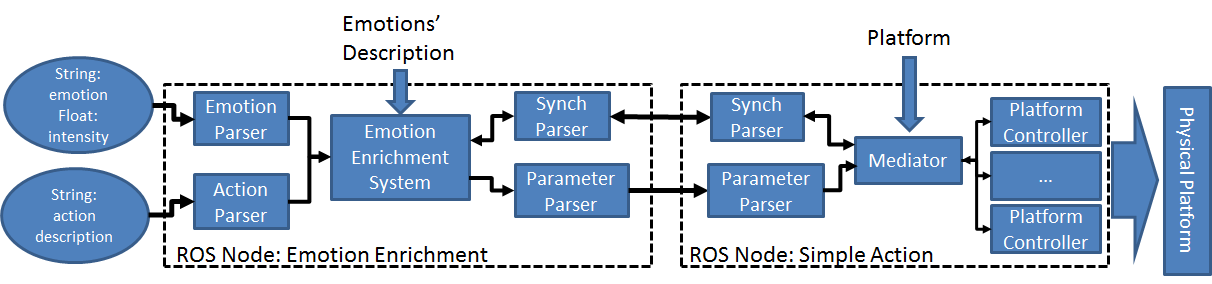
\includegraphics[width=1.0\textwidth]{Images/SystemArchitecture.png} 	
	\caption{General system design. Each simple action corresponds to one ROS node, and there is just one node for the emotion enrichment system. The ovals represent the ROS topic parameters, rectangles represent \textit{black boxes}, and texts outside containers represent input files that contain the system parametrization.}
	\label{fig:system_architecture}
\end{figure*}
The emotion enrichment core is divided in three different modules. 
Each module is responsible for one of the following phases:
\begin{enumerate}
	\item \textit{Generation of emotional execution tree:} this phase starts every time that a new action message is received. The process begins by parsing the format, verifying that the actions described on it exist in the system, and that the parameters correspond to the ones expected by each action included in the message. 
When the verification is done, and all the actions exist and the parameters correspond, an EXT such as the one presented in Figure~\ref{fig:emotional_enrichment} is created.
	\item \textit{Emotion addition:} uses the EXT created in the previous phase. In this phase new simple actions ($sa$)
can be added to the EXT, and the $sa$'s parameters are modified following the emotion description, which is loaded from files. This process is broken down in two steps. First, all the actions that are required to convey the desired emotion, and that are not yet present are added. Second, the emotional parameters are modulated basing on the emotion's intensity and character traits. The final EXT is presented in Figure~\ref{fig:reference}.
	\begin{figure}
		\centering
		%Representation
	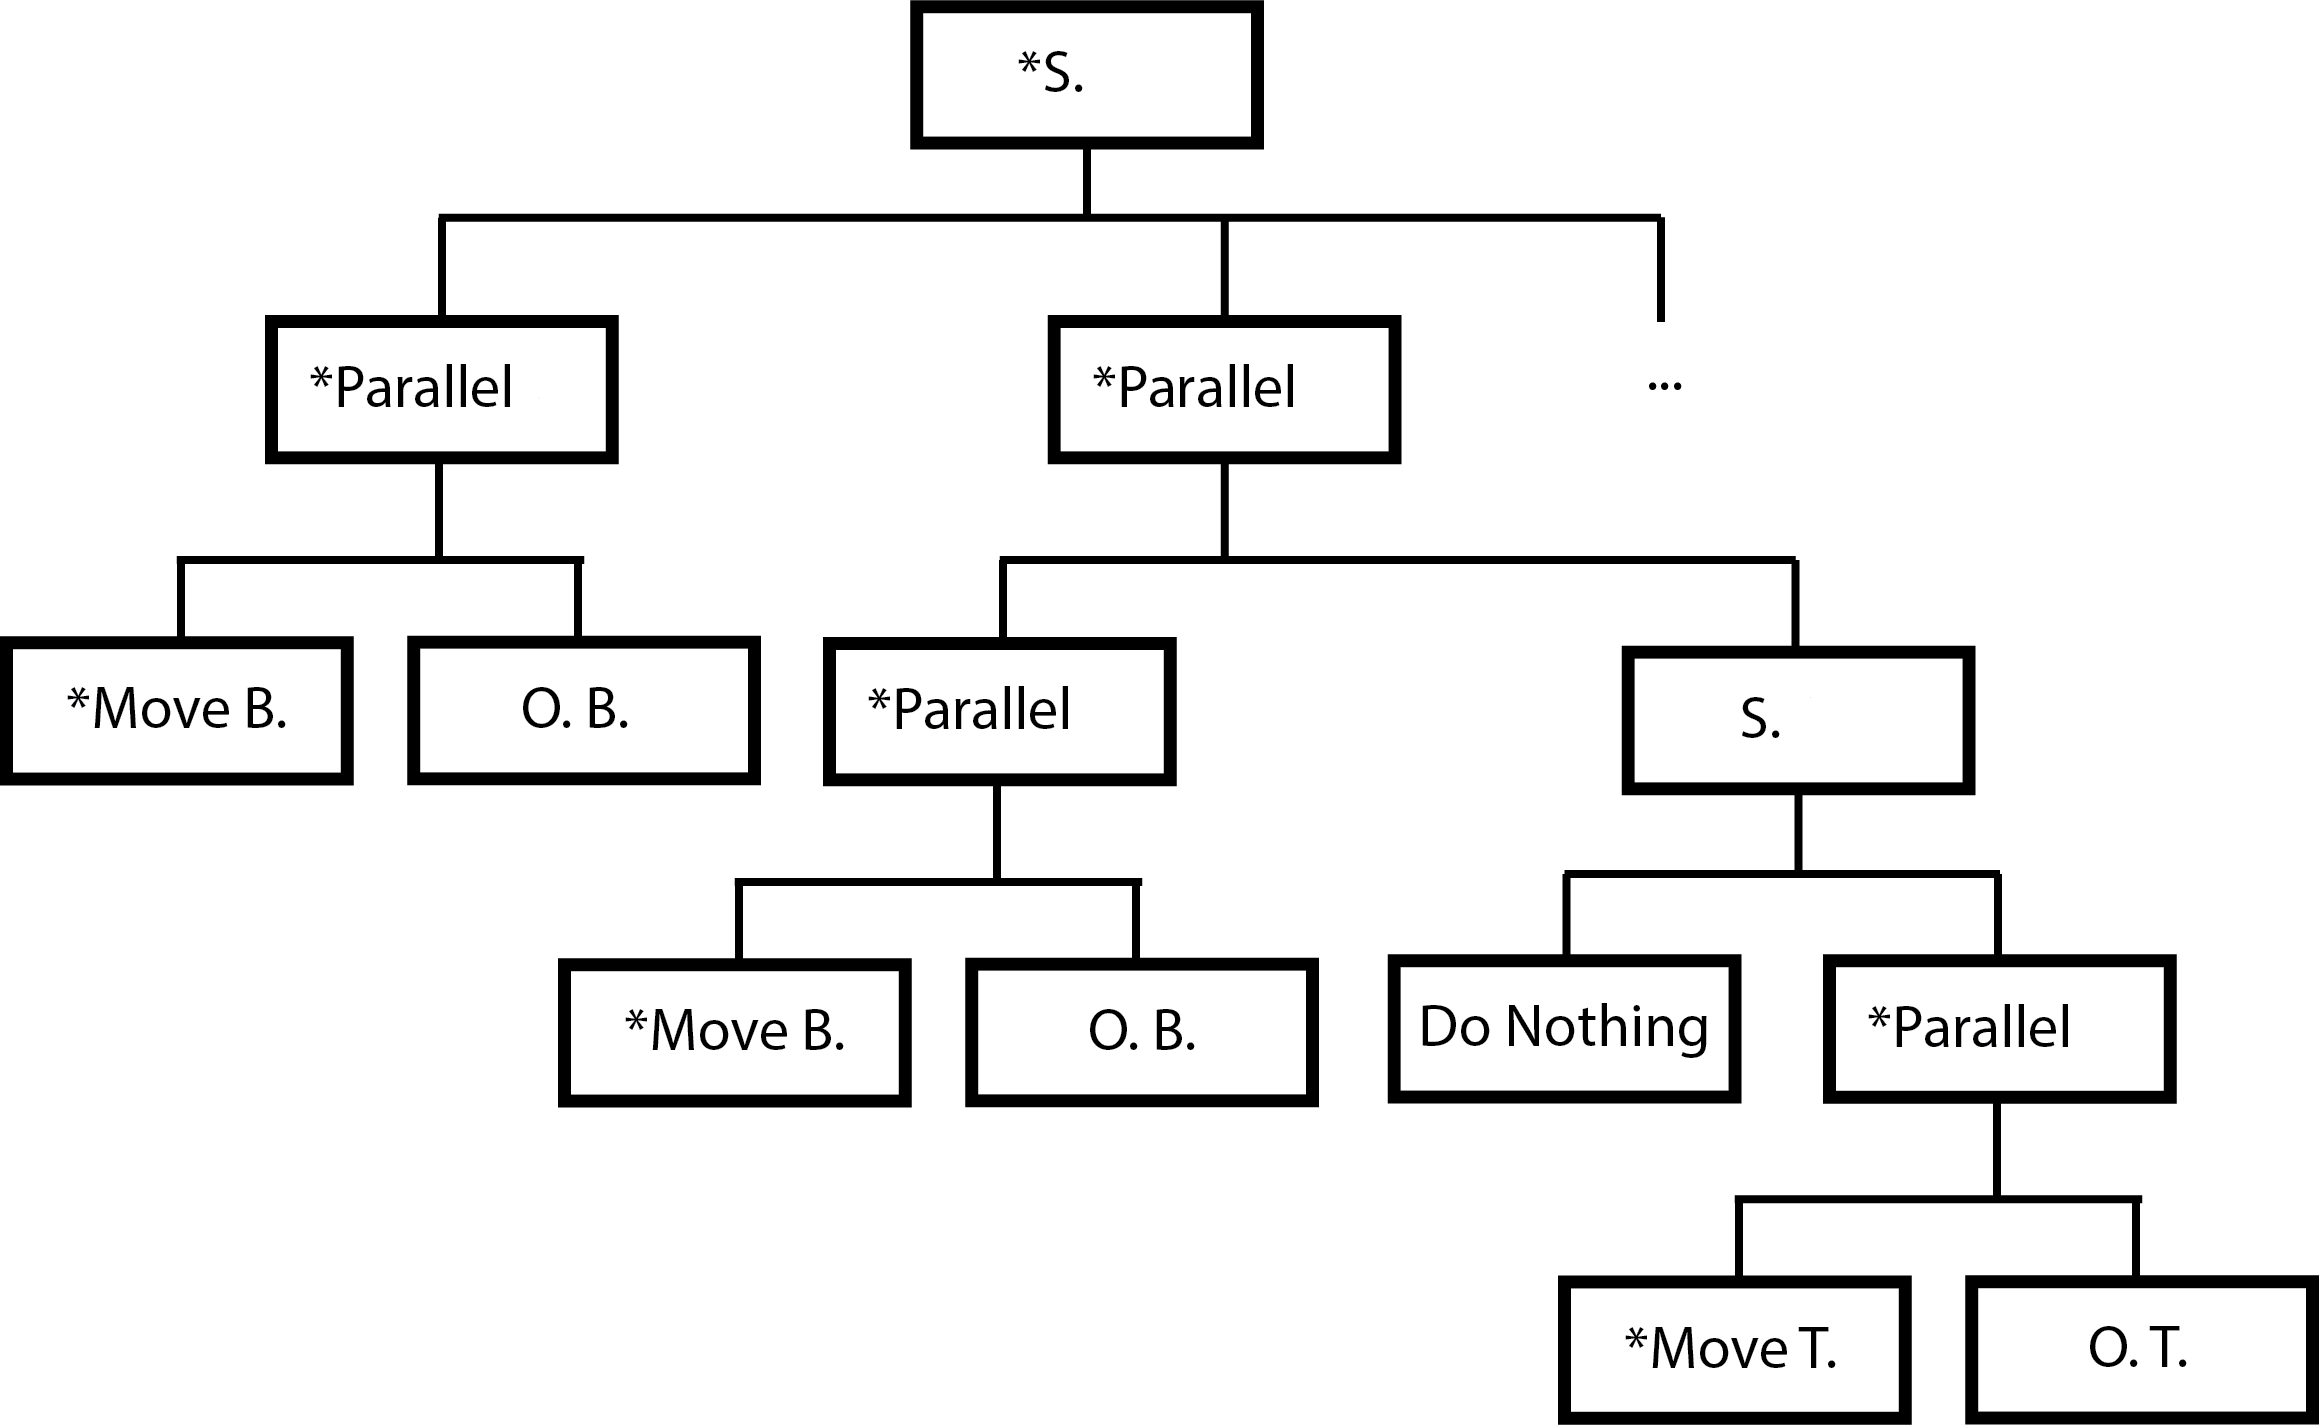
\includegraphics[width=0.45\textwidth]{./Images/exampleTreeE.png}
	\caption{EXT enriched with emotion for the EXT presented in Figure~\ref{fig:emotional_enrichment}.} 
	\label{fig:reference}
	\end{figure}
	\item \textit{Execution:} this is the last phase and it is done after the EXT is ''coloured'' with emotional characteristics (actions additions and emotional parameters). The decision to have two different communication channels, one for action parameters and another for the action emotional parameters, was taken to enable the possibility to update the emotional parameters without interfering with the current execution. 
\end{enumerate}

All the text message broadcast among the nodes are written using JSON format, which is human understandable, light, and can be parsed by many systems.
 
To test the system, two different platforms were used: Keepon Pro~\cite{Kozima–2009}
and an own made platform called Triskarino.
Keepon has been used to test the interoperability of the system to different platforms, while Triskarino has been used in diverse case studies to explore emotion projection with a non anthropomorphic platform.
%%%%%%%%%%%%%%%%%%%%%%%%%
%%%%%%%%%%%%%%%%%%%%%%%%%%%%%
\subsection{Keepon Test}
To test the system with Keepon (Fig.~\ref{fig:keepon}) was just necessary to implement the platform's controllers in each one of the simple action ROS nodes. Given that this platform does not have the capability to displace its body, the action move body was not implemented. Once added these controllers to the system, we proceeded to modify the configuration files to use this platform instead of Triskarino. With this small modification, we were able to change from one platform to other. In the video\footnote{YouTube video name Emotional Enrichment System, url: https://youtu.be/bRSXQ0rzkO8}
is shown the test where Keepon had to move its torso forward and backward to express a ``happy'' emotion. 
\begin{figure}
	\centering
	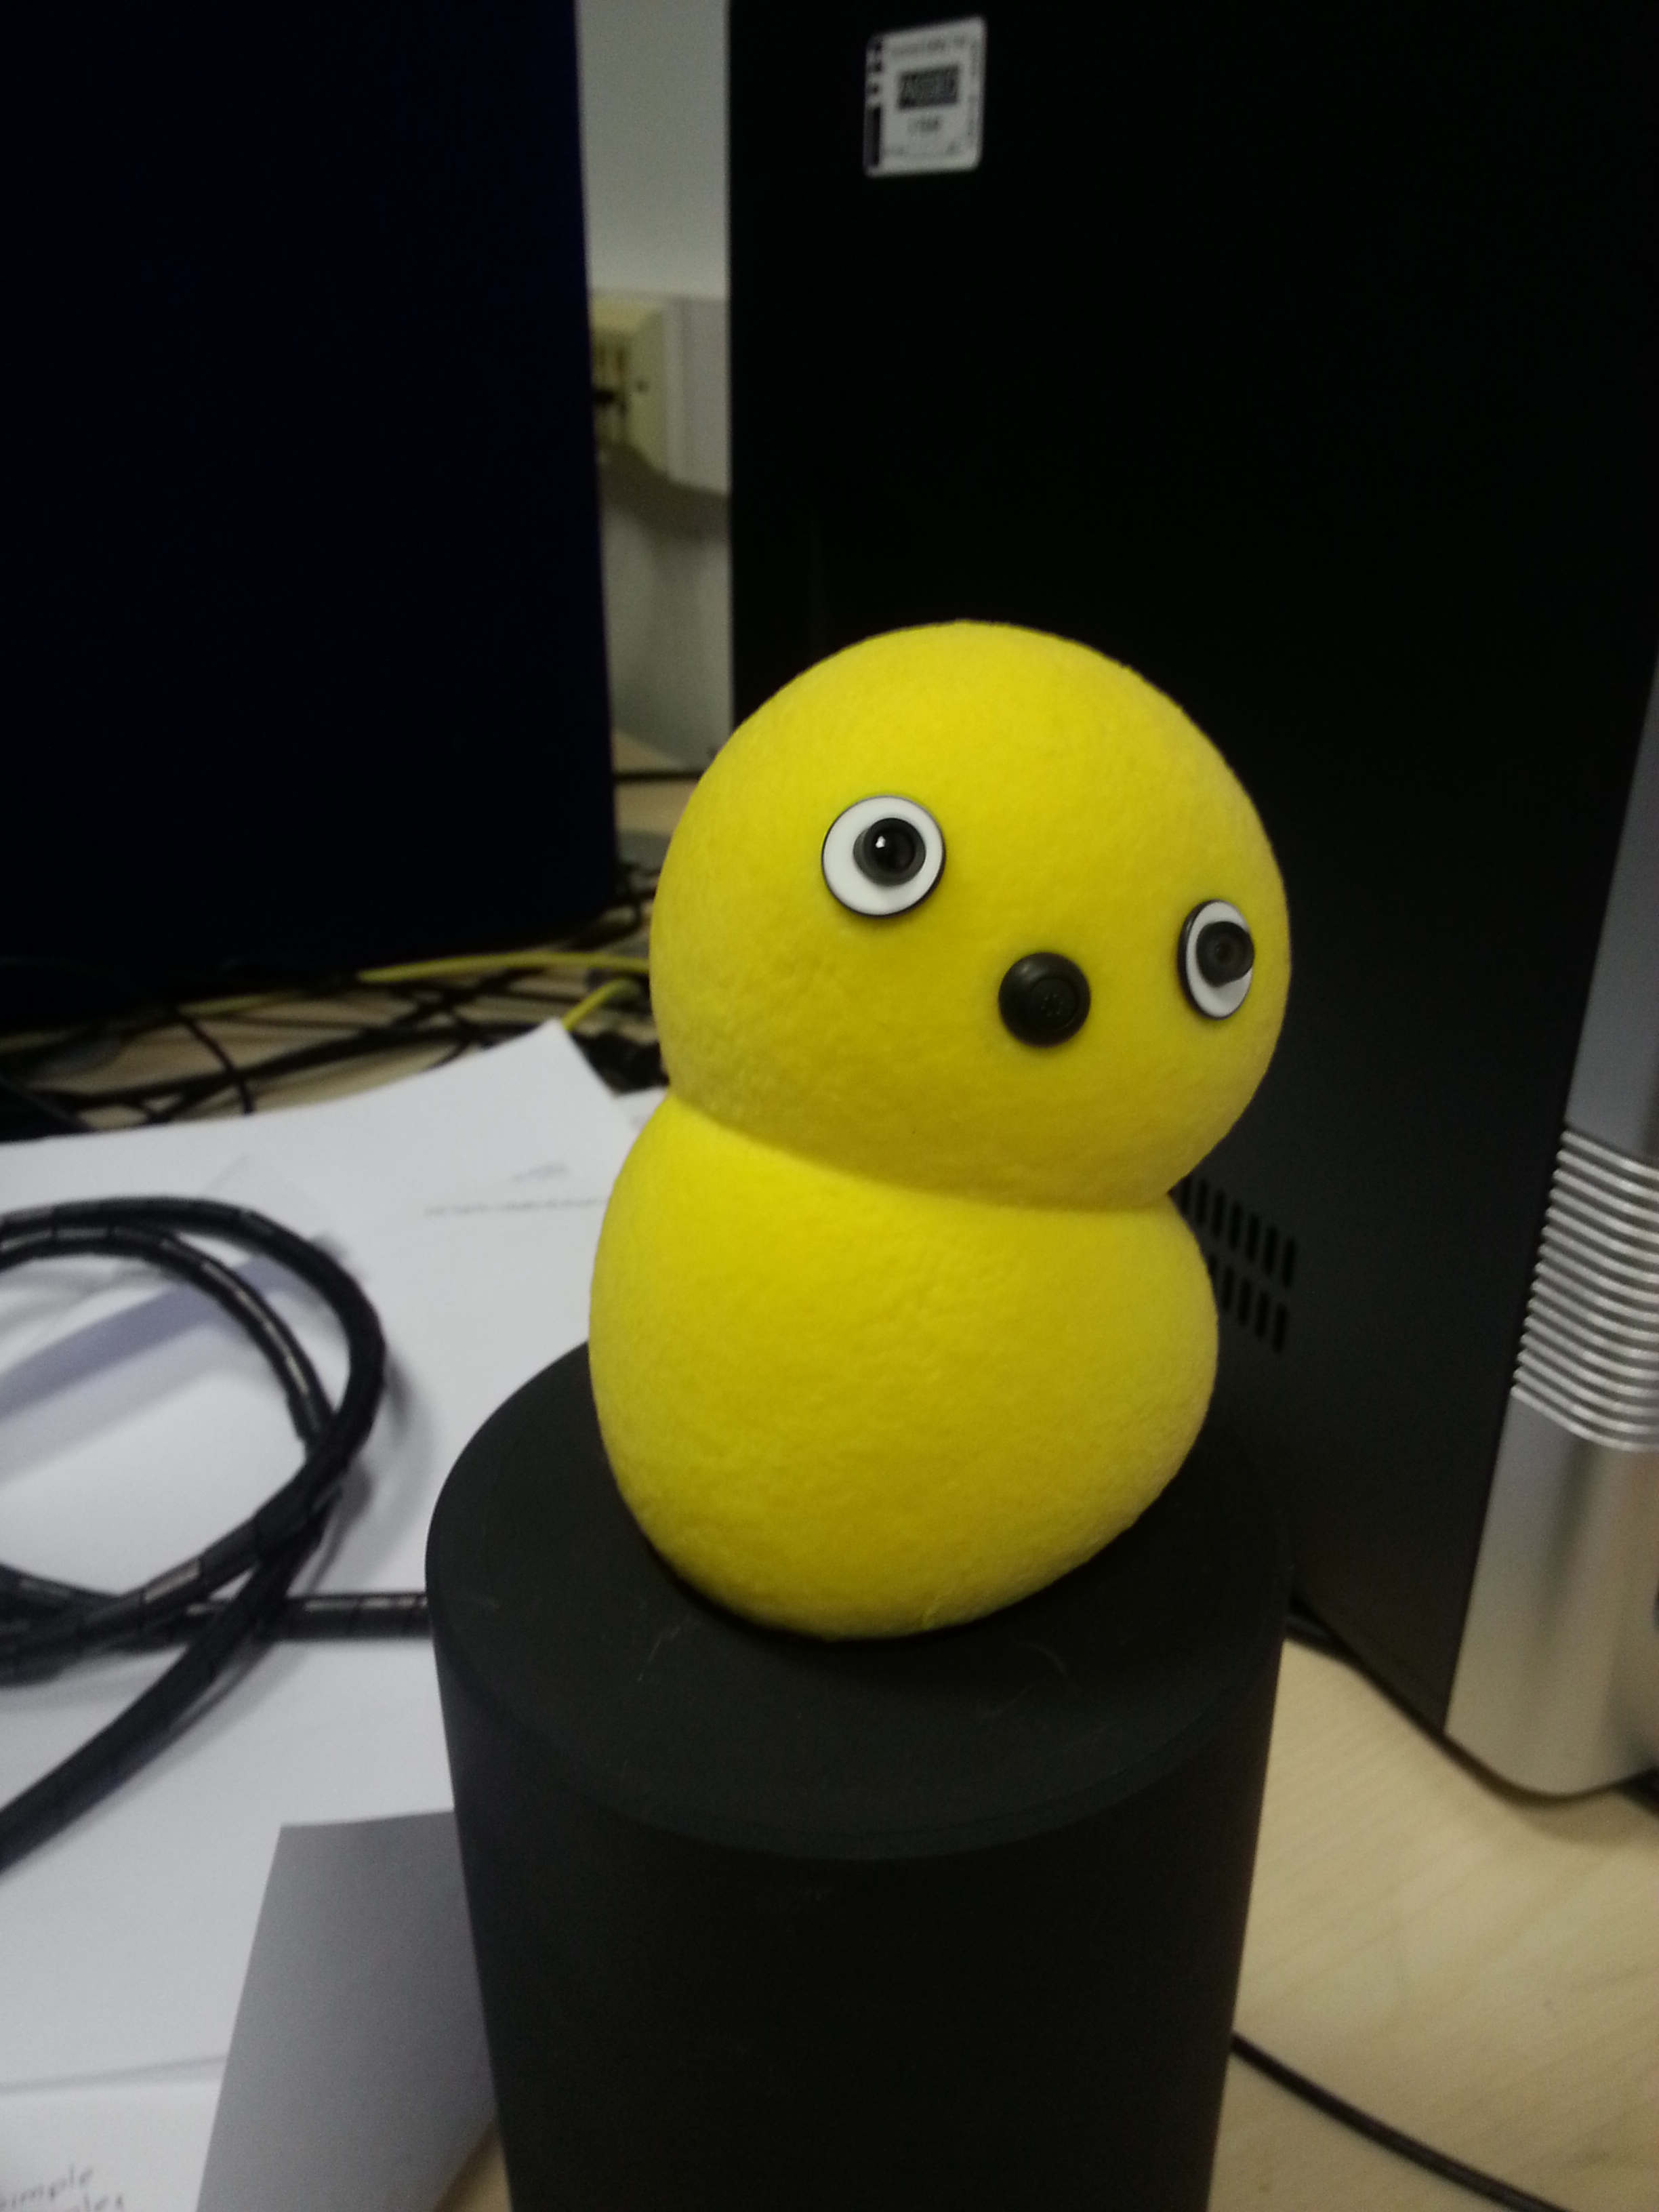
\includegraphics[width=0.2\textwidth]{./Images/Keepon.jpg}
	\caption{Keepon platform.}
	\label{fig:keepon}
\end{figure} 
The action is given by console telling the robot to bend the torso to a desired angle in x. The torso oscillation in y is added automatically by the system following the description given to happiness. 
 %%%%%%%%%%%%%%%%%%%%%
%%%%%%%%%%%%%%%%%%%%%%%%%%%%%
\subsection{Triskarino Test}
The system has been widely used with Triskarino (Fig.~\ref{fig:robot}) during our studies on projecting emotions with a non human like platform~\cite{angel2017robots}. 
\begin{figure}
	\centering
	\begin{subfigure}[c]{0.2\textwidth}
	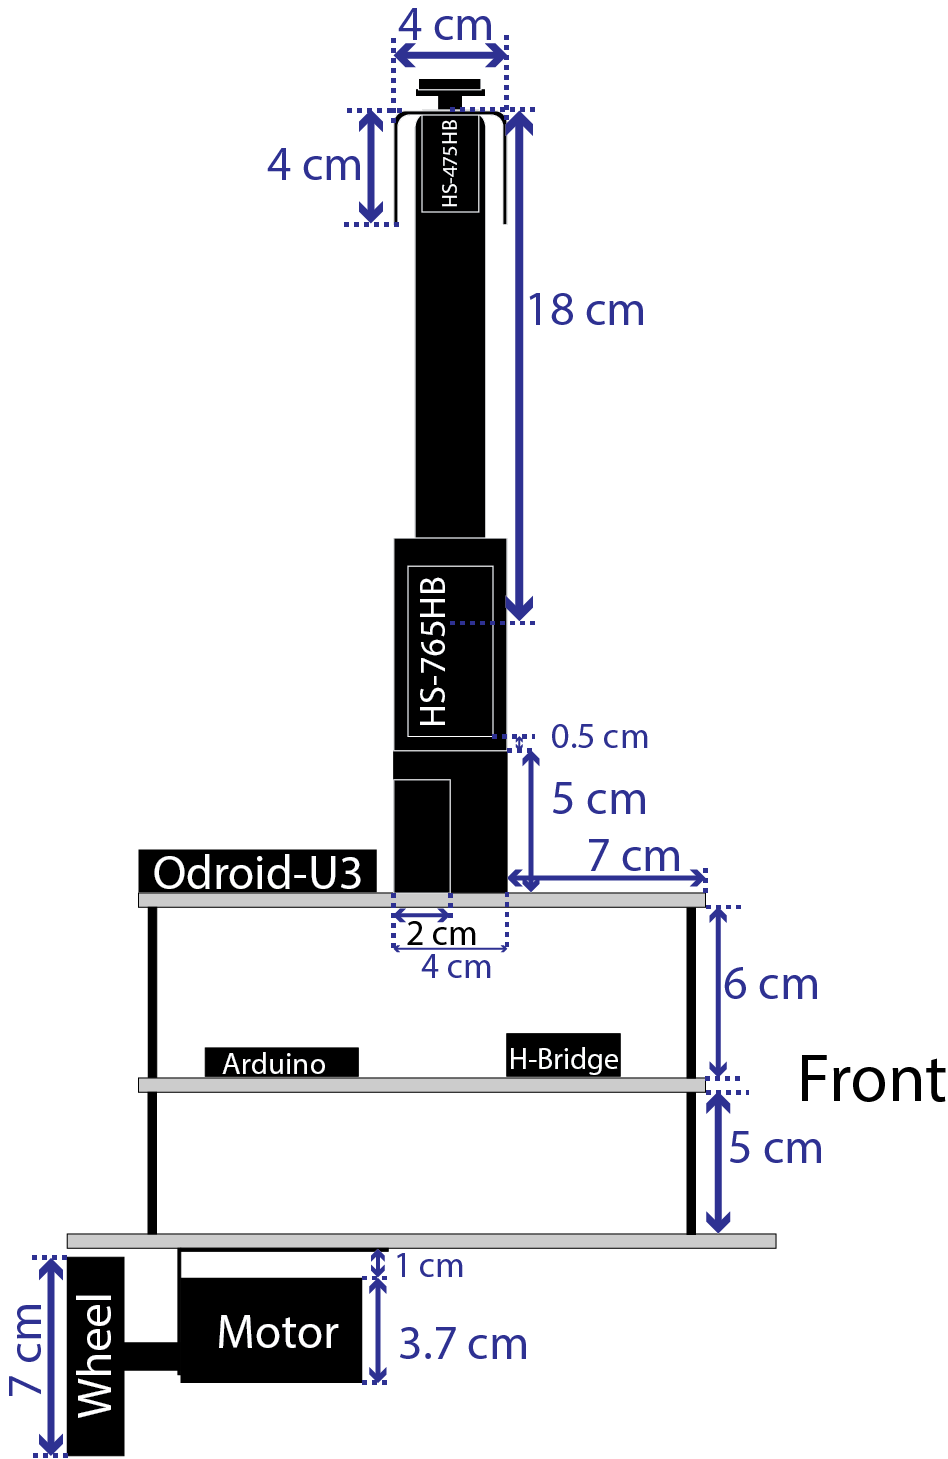
\includegraphics[width=\textwidth]{./Images/upperFourthD.png}
	\caption{Triskarino design.}
	\label{fig:design}
	\end{subfigure}
	\begin{subfigure}[c]{0.2\textwidth}
	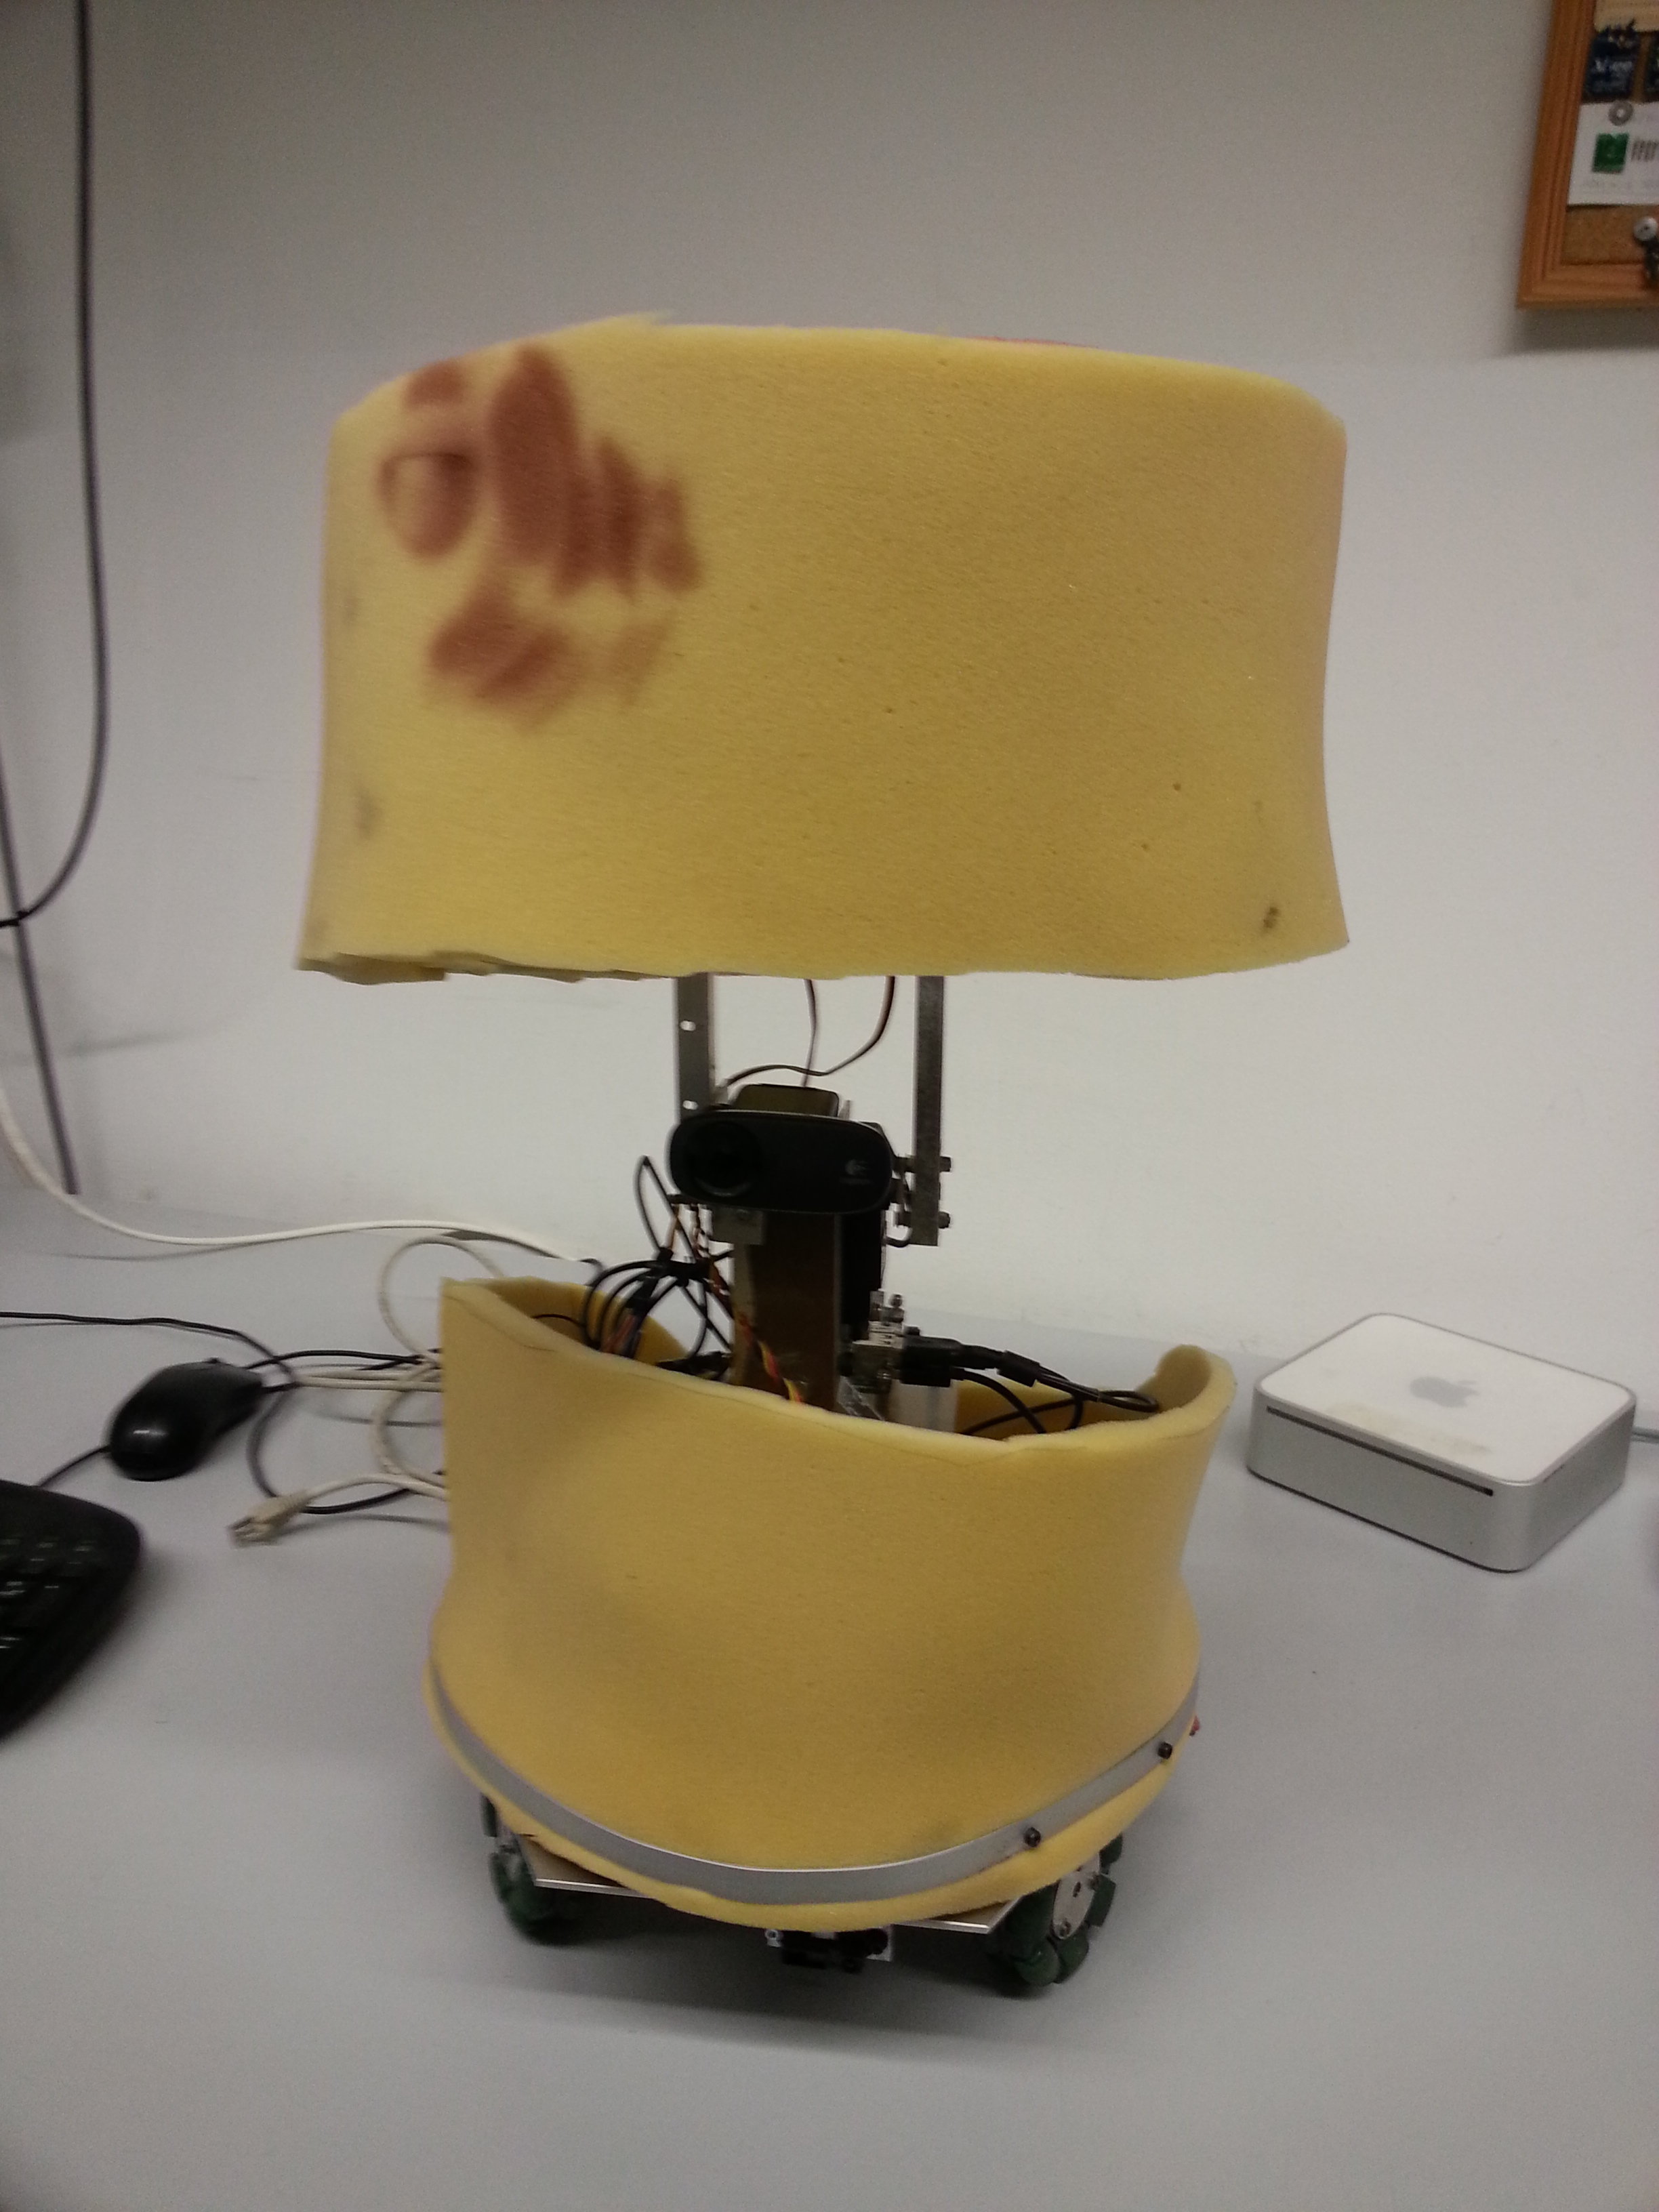
\includegraphics[width=\textwidth]{./Images/platform_fome.jpg}
	\caption{Triskarino with its cover.}
	\label{fig:triskar}
	\end{subfigure}
	\caption{Triskarino platform.}
	\label{fig:robot}
\end{figure}  
 During these studies the system was used in different experiments to move the robot on a straight line showing different emotions, each one selected from our command console. These studies were done in diverse events, such as Researchers' night and Maker Fair. Moreover, to show the whole capabilities of the emotional enrichment system and verify if could be used in real time, a little scene was set up. The scene is a modification of the first part of the balcony scene of Shakespeare's Romeo and Juliet play~\cite{RAndJ}.  The simplified sketch of our version could be seen in the Fig.~\ref{fig:triskar_test}. As it can be seen the stage was divided in 81 squares and the positions were given to the system in terms of the desire square to be reached, which allows the robot to adjust to the stage's dimension.
The whole sequence of actions were specified as unique action, having several sequential nodes and just move body action. The other actions, such as oscillate body or blend upper body were added online accordingly the desired emotion. 
